\frame{
\frametitle{Käynnistysjärjestelmä}
Polttomoottori ei käynnisty "itsestään"\ kuten höyrykone tai sähkömoottori.
\begin{itemize}
\item Tarvittava vääntömomentti määräytyy moottorin koon, rakenteen ja lämpötilan mukaan.
\item Nelitahtiottomoottorit vaativat 60--120 rpm käynnistysnopeuden, kaksitahtiset noin 200 rpm.
\item Dieselmoottoreilla noin 100 rpm, kammiomoottoreilla 120--200 rpm.
\item Ajoneuvokäytössä olevat moottorit käytännössä aina sähkömoottorikäynnisteisiä.
\item Käynnistimien nimellistehot vaihtelevat 0,3 kW -- 6 kW.
\end{itemize}
}

\frame{
\frametitle{Perusrakenne}
Käynnistysjärjestelmän pääosat ovat
\begin{itemize}
\item akku
\item virtalukko
\item käynnistin.
\end{itemize}
}

\frame{
\frametitle{Käynnistimen rakenne}
\begin{itemize}
\item Käynnistin koostuu moottorista, magneettikytkimestä ja hammaspyörästä kytkentälaitteineen.
\item Moottori on yleensä sarjamoottori tai kestomagneettimoottori.
\item Sarjamoottorin rakenne on yksinkertainen ja se tuottaa suuren momentin päällekytkentätilanteessa.
\item Moottori on yleensä 4- tai 6-napainen.
\end{itemize}
}

\frame{
\begin{center}
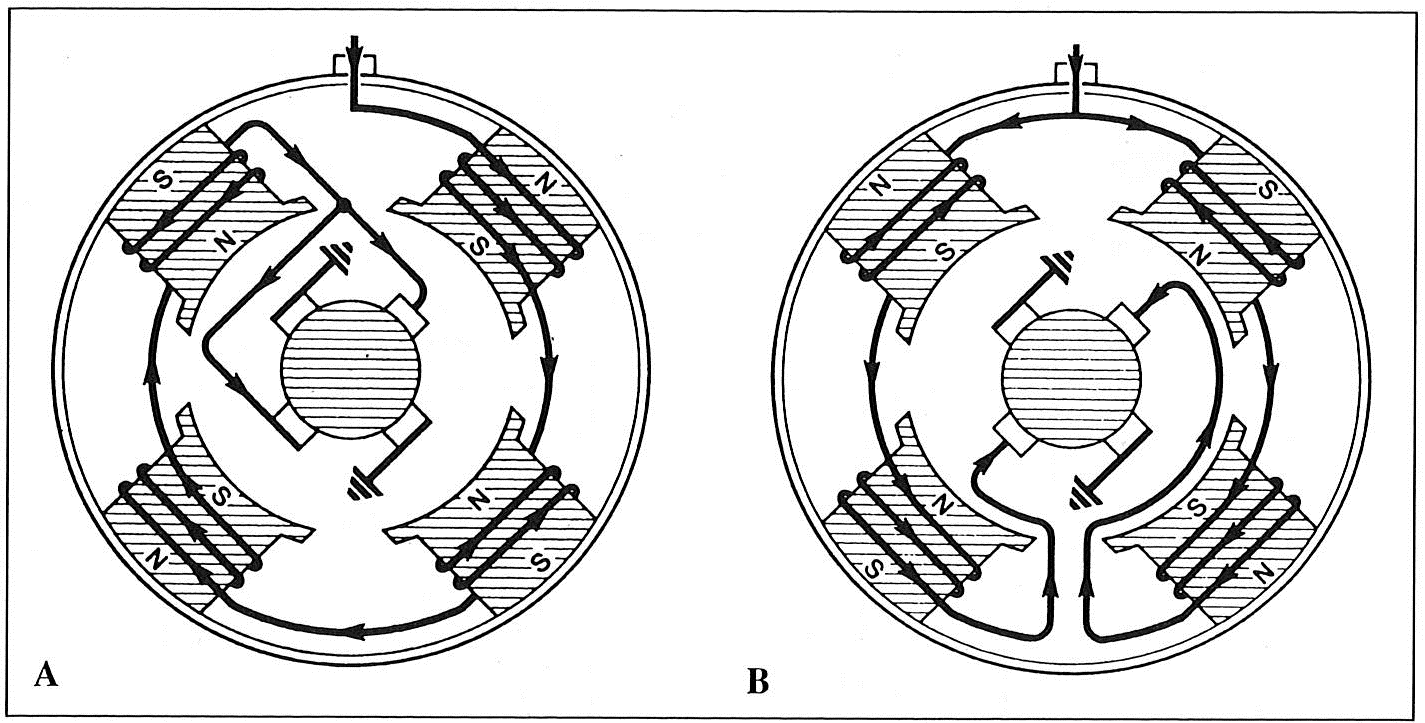
\includegraphics[height=60mm]{kaynnistysjarjestelma_pics/sarjamoottori.png}
\end{center}
\tiny Kuvan lähde: Juhala--Lehtinen--Suominen--Tammi: {\em Moottorialan sähköoppi}, 8. painos (2005), Autoalan koulutuskeskus, sivu 451.
}

\frame{
\frametitle{Hammaspyörien kytkentälaitteet}
\begin{itemize}
\item Käynnistinmoottorin akselilla oleva hammaspyörä pyörittää moottorin vauhtipyörällä olevaa hammaskehää.
\item Välityssuhde on tavallisesti 1:10--1:15.
\item Käynnistinmoottori kestää vain hyvin pieniä kierrosnopeuksia, joten se on pakko kytkeä irti moottorista käynnistyksen jälkeen.
\end{itemize}
}

\frame{
\frametitle{Hammaspyörien kytkentälaitteet}
Kolme päätyyppiä
\begin{itemize}
\item Magneettikytkimellä toimivat.
\item Käynnistimen hammaspyörän hitauteen perustuvat.
\item Siirtyvän ankkurin avulla toimivat.
\end{itemize}
}

\frame{
\frametitle{Kiertokäynnistin (vapaasiirtoinen kytkentähammaspyörä)}
\begin{itemize}
\item Perustuu hammaspyörän omaan hitauteen.
\item Käytetty vanhemmissa autoissa ja pienissä moottoreissa.
\item Kytkentähammaspyörä on kiinnitetty käynnistinmoottorin uritettuun akseliin.
\item Kun moottorin akseli pyörähtää, uritus työntää hammaspyörän akselin päähän ja kytkeytyy vauhtipyörään.
\item Kun moottori on käynnistynyt (=pyörii nopeammin kuin käynnistinmoottori), vauhtipyörän hammaskehä heittää 
hammaspyörän takaisin lähtöpaikkaansa.
\end{itemize}
}

\frame{
\frametitle{Työntökiertokäynnistin  (pakkosiirtoinen kytkentähammaspyörä)}
\begin{itemize}
\item Käytössä kevyessä ja keskiraskaassa kalustossa.
\item Magneettikytkin eli solenoidi työntää hammaspyörän vauhtipyörän hammaskehälle ja kytkee samalla käynnistinmoottoriin virran.
\item Hammasrattaan sisällä on vapaakytkin, joka suojaa käynnistysmoottoria rikkoontumasta välittömästi käynnistyksen jälkeen.
\end{itemize}
}

\frame{
\begin{center}
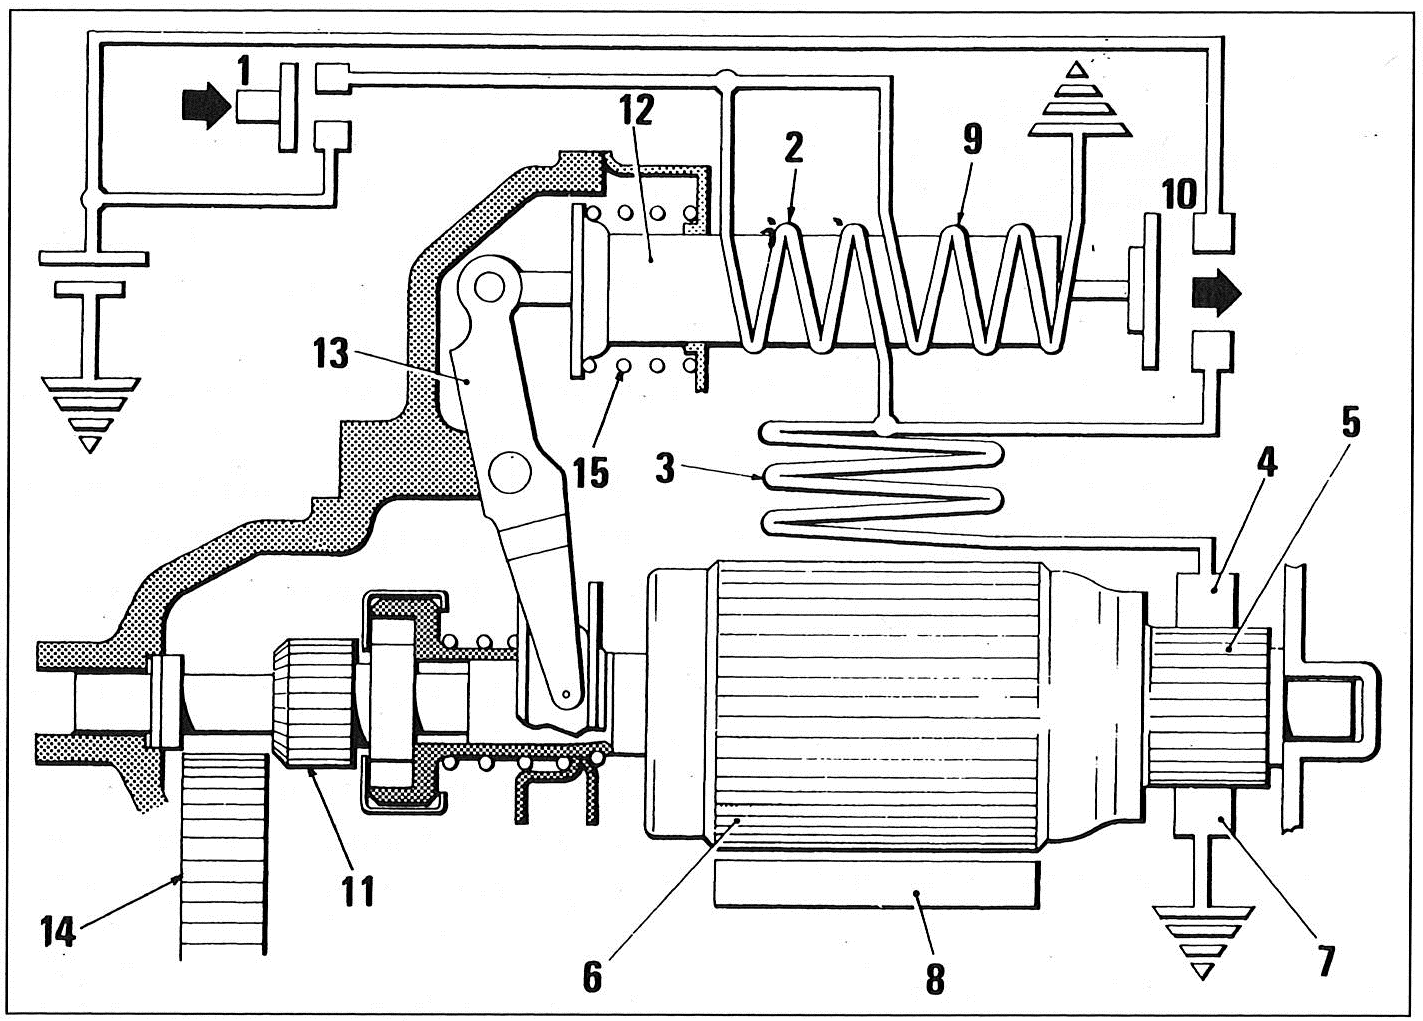
\includegraphics[height=80mm]{kaynnistysjarjestelma_pics/tyontokierto.png}
\end{center}
\tiny Kuvan lähde: Juhala--Lehtinen--Suominen--Tammi: {\em Moottorialan sähköoppi}, 8. painos (2005), Autoalan koulutuskeskus, sivu 453.
}

\frame{
\begin{center}
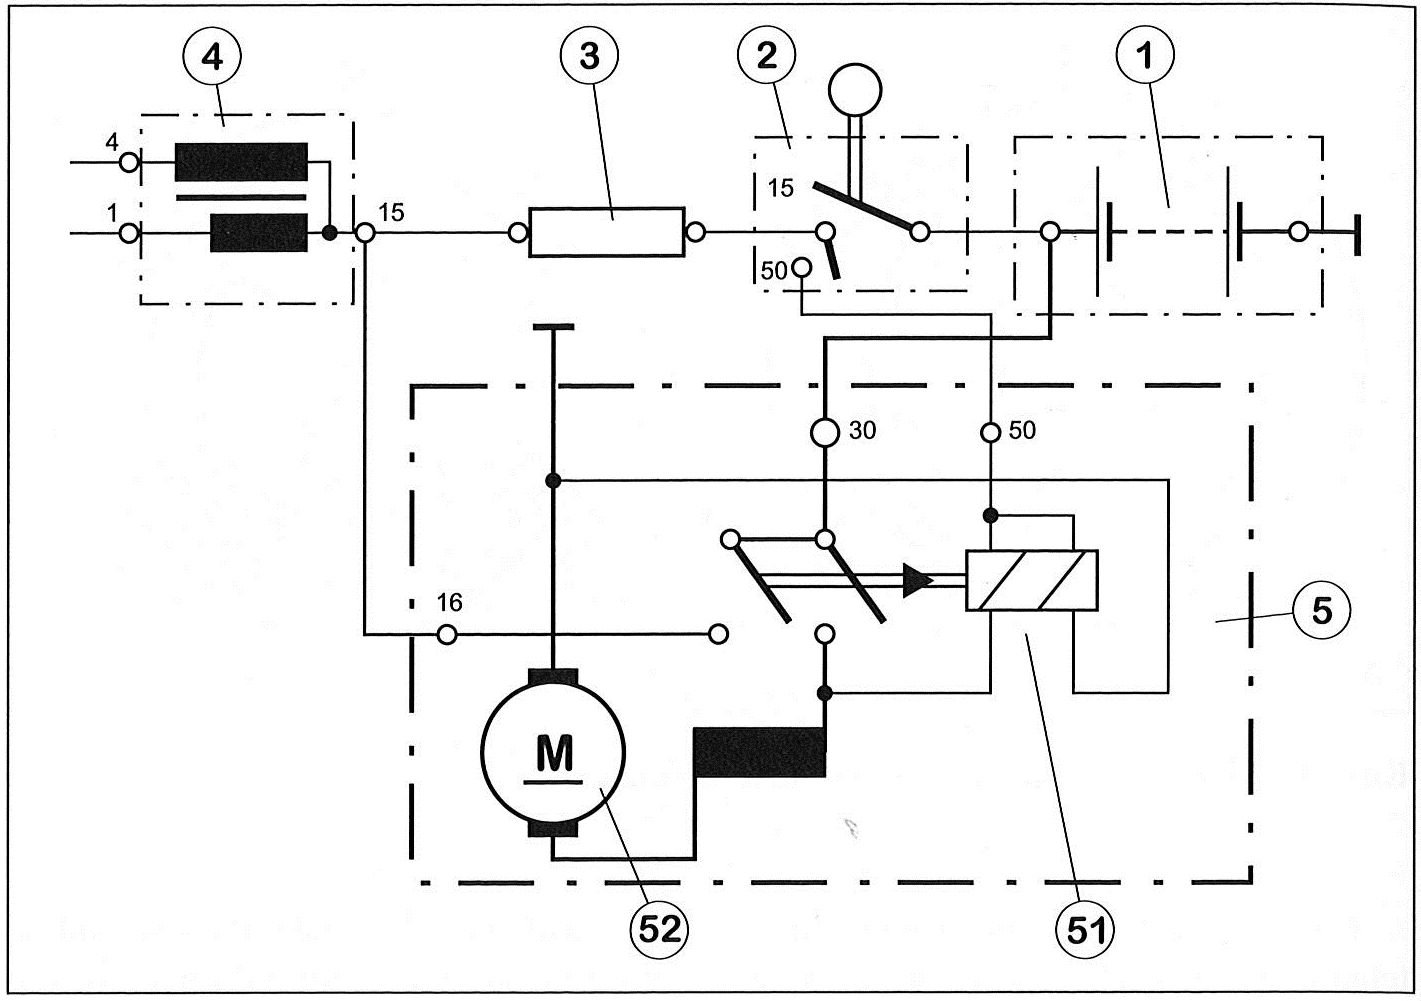
\includegraphics[height=80mm]{kaynnistysjarjestelma_pics/kytkis.png}
\end{center}
\tiny Kuvan lähde: Juhala--Lehtinen--Suominen--Tammi: {\em Moottorialan sähköoppi}, 8. painos (2005), Autoalan koulutuskeskus, sivu 452.
}

\frame{
\begin{center}
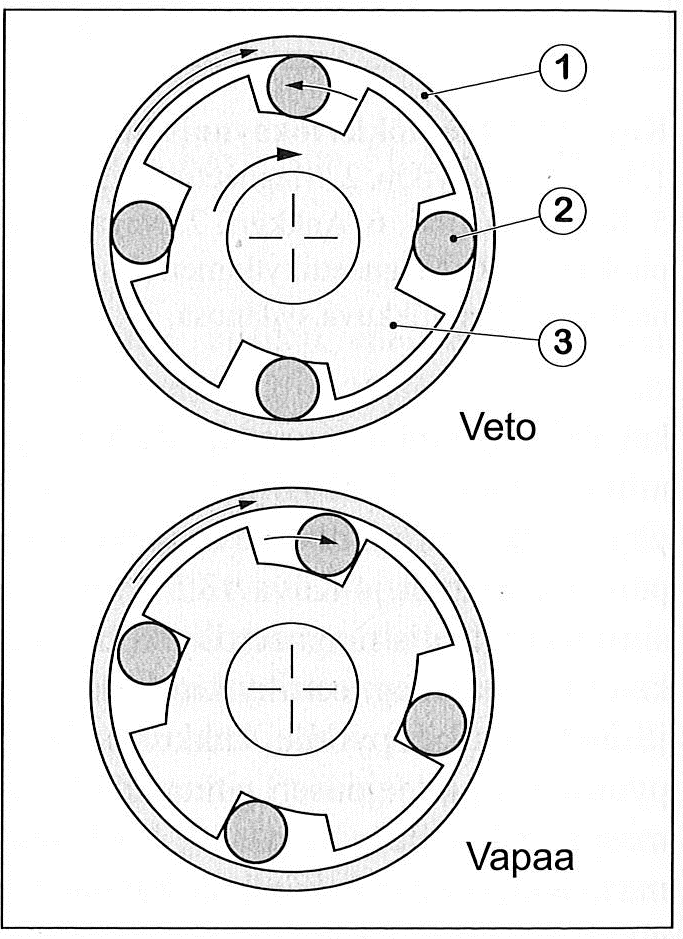
\includegraphics[height=80mm]{kaynnistysjarjestelma_pics/vapaak.png}
\end{center}
\tiny Kuvan lähde: Juhala--Lehtinen--Suominen--Tammi: {\em Moottorialan sähköoppi}, 8. painos (2005), Autoalan koulutuskeskus, sivu 454.
}

\frame{
\frametitle{Raskaan kaluston käynnistimet}
\begin{itemize}
\item Raskaissa dieselmoottoreissa vääntömomentin tarve on erittäin suuri.
\item Nykyään raskaassa kalustossa käytetään usein samaa tekniikkaa kuin pienemmissäkin moottoreissa.
\item Vanhemmissa kuorma-autoissa käynnistiminä käytettiin {\em työntöankkurikäynnistintä} ja {\em työntökäynnistintä}.
\item Keskiraskaissa moottoreissa käytetään {\em työntöankkurikäynnistintä}, joka toimii kuten työntökiertokäynnistin,
mutta siirtyvänä osana on koko moottorin ankkuri.
\item Hyvin suurilla käynnistystehoilla käytetään {\em työntökäynnistintä}, jossa solenoidi työntää onton akselin sisällä kulkevaan
tankoon kiinnitetyn hammaspyörän hammaskehäkosketukseen. Järjestelmässä on myös oma lamellikytkin, joka suojelee ankkuria
liian suurelta pyörimisnopeudelta ja momentilta.
\end{itemize}
Raskaat dieselmoottorit voidaan käynnistää myös paineilmalla, pienellä polttomoottorilla tai räjähdyspanoksella.
}

\frame{
\frametitle{Kestomagnetoitu käynnistin}
\begin{itemize}
\item Uusien voimakkaiden magneettien valmistustekniikan kehittyminen mahdollistaa kenttäkäämien
korvaamisen kestomagneeteilla. Etu: pienempi koko ja keveys.
\item Vääntömomentti on heikompi; tämä voidaan kompensoida pienellä vaihteistolla.
\end{itemize}
}

\frame{
\frametitle{Käynnistin-generaattori}
\begin{itemize}
\item Sama laite toimii sekä käynnistimenä että generaattorina.
\item Käytössä 50-70 -luvun pikkuautoissa, skoottereissa ja veneissä nimellä Dynastart.
\item Nykyään sama periaate hybridiautoissa: moottorin ja vaihteiston väliin on asennettu kestomagneettimoottori,
joka toimii myös vauhtipyöränä.
\item Ohjaus täysin elektroninen. Käyttöjännitteet vaihtelevat muutamista kymmenistä volteista aina 500 volttiin asti.
\end{itemize}
}


\frame{
\frametitle{Käynnistimen koestaminen}
Irrotettu käynnistin voidaan koestaa koestuslaitteessa.
\begin{itemize}
\item Joutokäyntikoe: käynnistimelle syötetään virtaa kuormittamattomana. Kuunnellaan sivuääniä ja luetaan virta ja jännite.
\item Kuormituskoe käynnistysnopeudella: käynnistintä jarrutetaan niin, että se pyörii käynnistysnopeudella. Tarkistetaan, että
jännite ja virta pysyvät ohjearvoissa.
\item Kuormituskoe lukittuna: käynnistin jarrutetaan pysähdyksiin ja luetaan jännite ja virta.
\end{itemize}
Kestomagneettimoottori voi tuhoutua jos se jarrutetaan lukkoon. Noudata aina valmistajan koestusohjeita.
}

\frame{
\frametitle{Käynnistimen kunnostus}
\begin{itemize}
\item Käynnistimen perusrakenne on yksinkertainen. Kunnostus ei eroa generaattorin kunnostamisesta: hiiliharjat, harjajouset ja käämitykset voidaan uusia.
\item Usein pääsee vähimmällä uusimalla koko käynnistimen.
\item Vauhtipyörän hammaskehä on tavallisesti kiinnitetty kutisteliitoksella ja se on vaihdettavissa.
\end{itemize}
}

\frame{
\frametitle{Dieselmoottorin hehkutuslaitteet}
\begin{itemize}
\item Vanhoissa autoissa hehkutus tapahtui erillisellä hehkutuskytkimellä.
\item 1970-luvulla käyttöön mekaanisella tai elektronisella lämpötilatunnistimella varustetut releet.
\item Nykyiset järjestelmät täysin elektronisesti ohjattuja.
\item Hehkutus voi alkaa jo, kun ovi avataan tai avain työnnetään virtalukkoon.
\item 2000-luvulla hehkutusrele korvattu tehotransistoreilla $\to$ pwm-säätö. Lisäksi tulppia ohjataan yksitellen.
\end{itemize}
}


\frame{
\frametitle{Hehkutusjärjestelmän vianhaku}
\begin{itemize}
\item Viallinen hehkutulppa on helppo löytää pihtivirtamittarin avulla.
\item Tulpan riittävä jännitteensaanti voidaan varmistaa mittaamalla akun plusnavan ja tulpan välinen jännite. Toimivassa järjestelmässä se on alle 1 V.
\end{itemize}
}

\frame{
\frametitle{Jäähdytysnesteen lämmittäminen hehkutulpilla}
\begin{itemize}
\item Uusissa etenkin pienikokoisissa dieselmoottoreissa terminen hyötysuhde voi olla niin hyvä, että jäähdytysnesteen lämpötila voi sopivissa olosuhteissa  jäädä niin alhaiseksi, että auton lämmityslaite ei toimi kunnolla.
\item Ongelma voidaan ratkaista lämmittämällä jäähdytysnestettä hehkutulppien avulla. Käytössä on myös polttoainekäyttöisiä lisälämmittimiä.
\item Lisälämmitys auttaa moottoria saavuttamaan toimintalämpötilansa nopeammin kylmäkäynnistyksen jälkeen.
\end{itemize}
}

% Kirjasta Nieminen: Auton sähkölaitteet sivu 154...
\frame{
\frametitle{Start-Stop -automatiikka}
\begin{itemize}
\item Kaupunkiajossa liikennevaloissa seisominen saastuttaa turhaan ilmaa ja kuluttaa polttoainetta.
\item Ratkaisu: pysäytetään moottori liikennevaloissa. Automatiikan tulee olla erittäin toimintavarma.
\item Start-Stop -järjestelmä pysäyttää moottorin, kun auto seisoo paikallaan, vaihde on vapaalla ja kytkinpoljin ylhäällä.
\item Kytkinpolkimen painaminen käynnistää moottorin välittömästi, jolloin autolla pääsee sujuvasti liikkelle.
\item Käynnistykseen voidaan käyttää myös generaattoria (lämmin moottori vaatii pienemmän momentin).
\item Start-Stop -järjestelmä voi vähentää polttoaineenkulutusta kaupunkiajossa yli 10 \%.
\end{itemize}
}

\frame{
\frametitle{Suorakäynnistys}
\begin{itemize}
\item Nykyaikainen suorasuihkutusmoottori on mahdollista käynnistää ilman käynnistintä.
\item Moottorinohjausjärjestelmä valitsee sylinterin, jossa mäntä on pysähtynyt sopivaan asentoon (työtahdin alkuosa).
\item Sylinteriin suihkutetaan polttoainetta ja annetaan kipinä => moottori pyörähtää käyntiin.
\item Esim. Mazda SISS (Smart Idle Stop System).
\end{itemize}
}